\documentclass{llncs}

\usepackage{llncsdoc}
\usepackage{graphicx,url}
\usepackage[brazil]{babel}
\usepackage[utf8]{inputenc}
\usepackage{float}
\usepackage{setspace}

\usepackage{tabularx}
\usepackage{cite}

\begin{document}
\sloppy
\title{Mezuro: Entendendo métricas de código}

\author{Diego de A. M. Camarinha\inst{1}, Rafael R. Manzo\inst{1},\\
        Daniel P. Alves\inst{1}, Daniel C. Bucher\inst{1}, \\
        Heitor R. Ribeiro\inst{1}, Paulo R. M. Meirelles\inst{2}}

\institute{Instituto de Matemática e Estatística -- Universidade de São Paulo (USP)\\
  Rua do Matão, 1010 -- 05508-090 -- Cidade Universitária -- São Paulo -- SP -- Brasil\\
  \email{\{diegoamc, manzo, danielpa, dbucher\}@ime.usp.br, \{heitor.ribeiro\}@usp.br}
  \and
  Faculdade do Gama -- Universidade de Brasília (UnB)\\
  Gama -- DF -- Brasil\\
  \email{paulormm@unb.br}}

\maketitle
\begin{abstract}
  % Contexto
  A facilidade de desenvolvimento e manutenção de um \textit{software} está diretamente relacionada com a qualidade de seu código fonte.
  % Problema
  % TODO: adicionar referência que apoie a falta de uso de análise estática em ambientes de desenvolvimento.
  No entanto, analisá-lo impõe dificuldades como, por exemplo, definir as métricas e interpretar o resultado de uma medição. Além disso, essa prática ainda não é comum em ambientes de desenvolvimento. Outro problema é a falta de ferramentas livres que integrem coletores de métricas para diversas liguagens.
  % Soluções propostas
  Neste artigo, apresentamos o Mezuro, uma plataforma \textit{web} livre para a avaliação colaborativa de código fonte. O projeto fornece um meio para comparar projetos e compartilhar conhecimento sobre métricas, ensinando a configurá-las e interpretá-las. A plataforma foi idealizada de forma que seja possível integrar diversos coletores de métricas para diversas linguagens. Atualmente, a ferramenta permite analisar códigos escritos nas linguagens C, C++, Java e Ruby.
  % Frase de impacto
  Com este projeto, esperamos disseminar o conhecimento e incentivar o uso de métricas de código.

\textbf{Palavras-chave:} análise estática, métricas de código fonte, \textit{software} livre.
\end{abstract}


\section{Introdução} \label{sec:intro}
Métricas de código-fonte estático são medidas extraídas a partir das análises léxica e sintática deste sem compilá-lo ou executá-lo e podem ser primitivas ou compostas, ou seja, formadas pela composição de uma ou mais métricas primitivas. Sua principal função é fornecer informações sobre complexidade, compreensão, testabilidade, manutenibilidade e evolução do código\cite{m13}.

Exemplos de métricas podem ser simples como linhas de código e quantidade de métodos por classe ou complexas como conexões aferentes de uma classe.
Hoje existem diversas ferramentas para a simples extração de métricas como  pylint\footnote{\url{http://www.pylint.org/}} (Python), metric\_fu\footnote{\url{https://github.com/metricfu/metric_fu}} (Ruby) e Analizo\footnote{\url{http://www.analizo.org/}} (C/C++ e Java), cada uma com diferentes graus de usabilidade, padrões e conjuntos de métricas, sendo necessária a criação de uma plataforma que reúna, organize e apresente essas informações para o usuário.

\section{Motivação}\label{sec:motivacao}
Por meio da avaliação de métricas de código-fonte podemos definir como está a qualidade do \textit{software} e pensar em estratégias interessantes para lidar com a chamada ``crise do \textit{software}'' \cite{nr68}. Esta afirma que, com o crescimento da capacidade computacional, mais problemas difíceis passam a ter solução viável, mas que, por outro lado, a complexidade da interface para uso dos novos equipamentos (\textit{hardware}) e do processo de desenvolvimento atuais combinados com a complexidade dos problemas exacerbam falhas do \textit{software}. Assim, o controle da qualidade de um \textit{software} durante sua evolução no tempo torna-se uma ferramenta para identificar e prevenir tais falhas.

Porém, incorporar esta avaliação às metodologias de desenvolvimento de \textit{software} não pode ser um processo manual em razão do risco desta prática cair em desuso. Isto se deve ao fato de que as ferramentas de extração de métricas, em geral, não apresentam uma interface amigável para seres humanos lerem seus resultados e muito menos um padrão entre si.
Neste contexto, uma ferramenta com as seguintes características se faz necessária para a introdução deste tipo de avaliação constante às metodologias:
\begin{itemize}
  \item interface que agrupe as diversas ferramentas disponíveis;
  \item permita seleção e composição de métricas de forma flexível;
  \item manutenção de um histórico de evolução;
  \item exiba os resultados de forma amigável.
\end{itemize}

Por último, como explicado por Meirelles \cite{m13}, ainda não existe um consenso sobre qual conjunto de métricas é relevante para se avaliar a qualidade do código e muito menos quais valores destas supostas métricas são bons ou ruins. Portanto, mais uma característica interessante para uma ferramenta neste campo é que permita aos usuários especialistas definirem tais parâmetros, viabilizando estudos estatísticos que nos aproximem de uma conclusão.

\section{Ferramentas similares}
Foram levantadas informações básicas sobre duas ferramentas similares já consolidados dentre desenvolvedores de \textit{software} para que possamos avaliá-las brevemente com respeito aos critérios definidos na motivação (seção \ref{sec:motivacao}).

A primeira delas e mais próxima do idealizado, o SonarQube\footnote{\url{http://www.sonarqube.org/}} é um \textit{software} livre, licenciado como LGPLv3, que oferece uma plataforma de gerenciamento de qualidade de código. Por meio de \textit{plugins} disponíveis através de uma biblioteca\footnote{\url{http://docs.codehaus.org/display/SONAR/Plugin+Library/}}. Em sua versão básica ele classifica problemas encontrados no código e calcula métricas simples de cobertura de testes e divida técnica em várias linguagens. Entretanto, seus melhores \textit{plugins} tem código fechado e pago como, por exemplo, o para análise de C/C++\footnote{\url{http://www.sonarsource.com/products/plugins/languages/cpp/}}.

Por sua vez, o Code Climate\footnote{\url{https://codeclimate.com/}} é uma ferramenta que fornece análise de códigos JavaScript ou Ruby (da versão 1.8 em diante) que estejam disponíveis em um servidor Git.

O \textit{software} procura por ``\textit{code smells}'' no programa do usuário e os classifica como mais ou menos problemáticos levando em consideração o tamanho dos métodos e duplicação de blocos. Conforme os encontra, o programa atribui valores ao código para no final determinar uma nota de \textit{A} a \textit{F} com base no somatório dos valores encontrados. Note que a análise feita não necessariamente indica um problema real, uma vez que aquela pode ter sido a implementação escolhida pelo programador.

Recentemente, o Code Climate iniciou uma análise estatística preliminar de todos os projetos que já foram analisados por este. Publicada informalmente em uma simples publicação em sua página\footnote{\url{http://blog.codeclimate.com/blog/2014/05/21/does-team-size-impact-code-quality/?utm_source=Code+Climate&utm_campaign=69c024549d-newsletter-NI-2014-05-22&utm_medium=email&utm_term=0_672a7f5529-69c024549d-317410425}}.

\section{Mezuro}\label{sec:mezuro}
Nesta seção, apresentaremos o projeto Mezuro\footnote{\url{http://mezuro.org}}. Explicaremos o contexto no qual o projeto foi criado, mostrando como as ideias das partes que o compõe evoluíram até alcançar o estágio atual. Além disso, descreveremos a integração do projeto com o Noosfero\footnote{\url{http://noosfero.org}} e porque ela não deu certo. Por fim, exibiremos a fase atual de desenvolvimento de todas as partes do Mezuro, explicitando as decisões mais importantes que foram tomadas para melhorar o andamento do projeto.

\subsection{Histórico}\label{sec:historico}

\subsection{Integração com o Noosfero}\label{sec:noosfero}

\subsection{Mezuro \textit{standalone}}\label{sec:standalone}

O projeto Mezuro, com forte viés acadêmico, visa ser uma interface que permita, de forma flexível, a extração e análise de métricas estáticas de código-fonte, licenciado como \textit{Affero General Public License} versão 3 (AGPLv3). Nele, o usuário é o responsável por definir o conjunto de métricas a ser utilizado para realizar cálculos, com a possibilidade de armazenar os resultados para comparações futuras. Seu objetivo é:
\begin{itemize}
    \item Aproximar-se de um consenso acerca de quais métricas devem ser empregadas na análise da qualidade de um código-fonte;
    \item Buscar os valores destas métricas que definem a qualidade de um código-fonte.
\end{itemize}
\subsection{Reescrita}
Nos últimos meses de 2013, foi encontrado um problema no Prezento, impossibilitando que o projeto seguisse em frente, entrando em um estado de estagnação. Na seqüência, foram realizados diversos testes na esperança de localizar o que estava causando o comportamento indesejado, até que, finalmente, foi descoberto que este estava relacionado aos processamentos da Kalibro. A partir deste ponto, sucessivas tentativas de debug tomaram conta da rotina do Mezuro, todas sem sucesso, uma vez que o a arquitetura monolítica da Kalibro tornava a manutenção do seu código extremamente complicada. Assim, foi levantada a questão de reescrevê-la em Ruby. Porquê Ruby? Dentre muitos motivos, os principais foram a familiaridade da equipe com a linguagem e o fato de que o resto do Mezuro já estava escrito em Ruby. 
Como já estávamos perdendo um tempo relativamente alto com o problema, não foi difícil optarmos pela opção ``um passo para trás, dois para frente'', pois já pensávamos nos lucros que teríamos com a reescrita, sem mencionar os temores que tínhamos se não optassemos por ela, como por exemplo encontrarmos outros problemas de tão difícil resolução quanto o que já tinhamos em mãos. Nos meses seguintes, após tomada a decisão (a esta altura já estávamos no início de 2014), começamos a adaptar todo o projeto para receber a mudança e começarmos efetivamente a reescrita da Kalibro. 
Com dedicação total da equipe, o processo de reescrita demorou do final de Maio ao final de Agosto de 2014 e, melhor que isso, o problema que tínhamos com a antiga Kalibro foi resolvido e hoje temos uma base de processamentos estável com um código de fácil manutenibilidade.

  \subsection{Arquitetura}
  Com o objetivo de ser agradável para o desenvolvedor, buscamos criar um sistema de simples manutenção que incorpore outras funcionalidades facilmente. Para isto, visamos:
  \begin{itemize}
    \item Minimizar a quantidade de código a ser mantida;
    \item Testar e garantir a qualidade do código;
    \item Modularizar a aplicação em diversos serviços independentes.
  \end{itemize}

  A figura \ref{fig:architecture-1} especifica o atual estado do Mezuro:
  \begin{figure}[H]
    \centering
    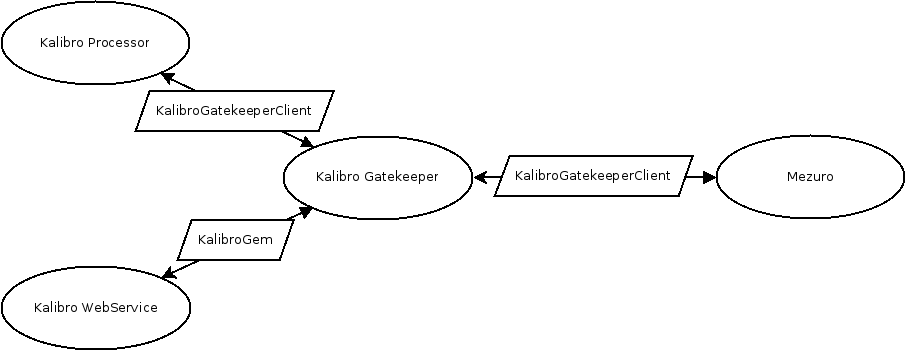
\includegraphics[width=\textwidth]{images/mezuro-architecture-actual.png}
    \caption{Arquitetura atual do sistema.}
    \label{fig:architecture-1}
  \end{figure}
  As elipses são os diferentes \textit{softwares} envolvidos e os paralelogramos as interfaces de comunicação entre eles. Na base do Mezuro encontra-se o Kalibro, segmentado em três entidades menores, como ilustrado na figura \ref{fig:architecture-2}:
  \begin{figure}[H]
    \centering
      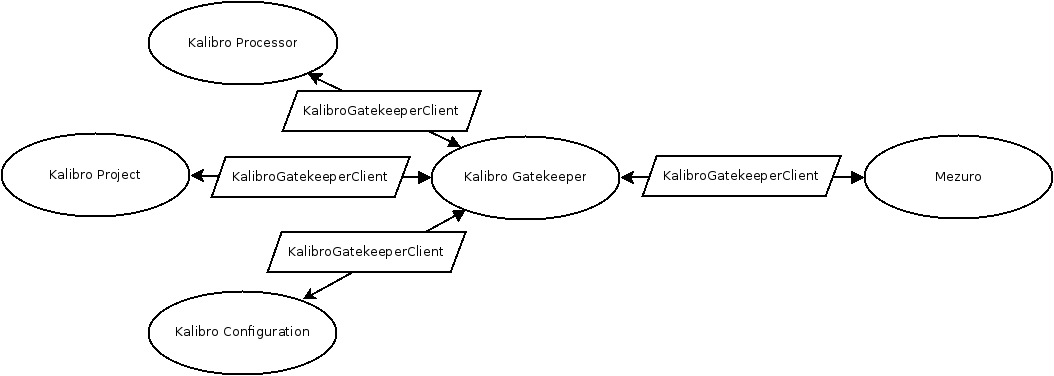
\includegraphics[width=\textwidth]{images/mezuro-architecture-predicted.png}
    \caption{Arquitetura futura do sistema.}
    \label{fig:architecture-2}
  \end{figure}
  O objetivo pretendido com quebra da estrutura monolítica do Kalibro é que sua manutenção e evolução torne-se mais fácil, sem que todo o sistema seja comprometido.

  \subsection{Diferenciais} \label{subsec:motivacao}
  As principais motivações para o surgimento de uma ferramenta como o Mezuro são os seguintes problemas:
  \begin{itemize}
      \item Não há parâmetros de comparação consolidados entre projetos;
      \item Existem estudos, mas poucos dados empíricos;
      \item Ainda é dada pouca importância ao monitoramento de código.
  \end{itemize}

  \subsection{Por que usar o Mezuro?} \label{sec:projeto-mezuro}
  Idealizado como uma plataforma de métricas de código, um dos diferenciais do Mezuro reside na possibilidade de gerar informação sobre o código-fonte de forma contínua: o usuário decide quando analisar novamente o projeto e acompanha detalhadamente a evolução das notas ao longo do tempo. Os resultados de cada análise são públicos, o que permite uma maior transparência entre o desenvolvedor e a comunidade que utiliza aquele \textit{software}. Assim, ela pode decidir se aquela solução atende ou não às suas necessidades e se deve depositar confiança na qualidade do \textit{software} desenvolvido.

  \subsection{Principais funcionalidades}\label{sec:princ-funcionalidades}
  No Mezuro, as funcionalidades podem ser divididas em dois grupos:
  \begin{itemize}
    \item Projeto
      \begin{itemize}
      \item \textit{Download} do código-fonte a partir de repositórios (Git, Subversion, Bazaar etc) ou via arquivo compactado;
          \item Escolha da periodicidade do processamento do código (1 dia, 2 dias, semanal, quinzenal e mensal);
          \item Escolha de qual configuração de métricas cada repositório irá utilizar;
          \item Nota de cada métrica da configuração para cada arquivo do repositório;
          \item Análise gráfica de cada arquivo do repositório por meio de um gráfico de pontos com notas ao longo do tempo;
          \item Resultados públicos e acessíveis à comunidade.
      \end{itemize}
      \item Configuração
      \begin{itemize}
      \item Criação de configuração e a possibilidade de clonagem;
          \item Estatísticas sobre as configurações mais populares dentro da comunidade;
          \item Criação de intervalos qualitativos associados aos valores das métricas;
          \item Criação de grupos de leitura para a interpretação textual dos resultados das métricas;
          \item Combinações de métricas nativas para criação de análises compostas e mais complexas.
      \end{itemize}
  \end{itemize}

  \subsection{A rede social}\label{sec:user-potencial}
  O Mezuro tem o formato de uma rede social, no qual os participantes podem ver a produção de terceiros por meio da avaliação dos projetos ou do clone das configurações. Essa interação mútua e aberta pode ser interessante para desenvolvedores, gerentes de projeto, auditores de \textit{software} e até mesmo uma equipe de desenvolvimento inteira. O objetivo final é criar uma comunidade que veja o valor de tais metodologias e como isso pode contribuir para o sucesso do seu projeto.

  \subsection{Casos de uso}
  Apresentaremos a seguir as duas principais funcionalidades da ferramenta ilustradas por meio de capturas de telas. Em todas elas, utilizamos uma conta já cadastrada no sistema (único privilégio necessário para realizá-las).

    \subsubsection{Criação de configuração}
    \begin{figure}[H]
      \centering
      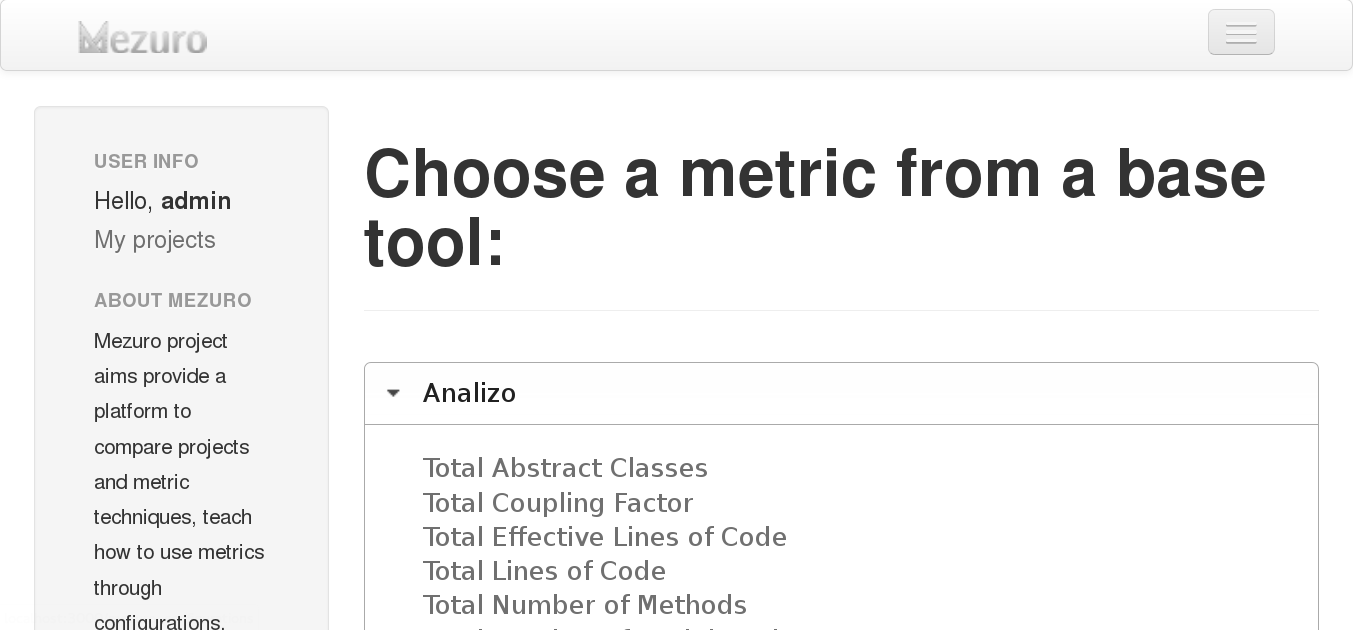
\includegraphics[width=\textwidth]{images/choose-metric.png}
      \caption{Interface para escolha de ferramenta extratora de métrica e escolha de uma métrica nativa para adicionar a uma configuração.}
      \label{fig:choose-metric}
    \end{figure}

    Criar uma configuração envolve 5 telas do sistema em 4 passos básicos:
    \begin{enumerate}
      \item Acessar a página de listagem de configurações;
      \item Clicando em ``New configuration'', preencher o formulário de criação de configuração e salvá-lo;
      \item Clicando em ``Add metric'', escolher a ferramenta de extração e qual métrica a ser usada (figura \ref{fig:choose-metric});
      \item Preencher o formulário (detalhado a seguir) e salvá-lo.
    \end{enumerate}

    Os passos 3 e 4 devem ser repetidos para cada métrica adicionada à configuração. O formulário de métrica (passo 4) é complexo se comparado ao de configuração mas, assim como os demais, cada campo possui detalhes sobre sua utilização. Aqui, destacamos os menos evidentes:
    \begin{itemize}
      \item \textbf{Aggregation Form:} Maneira com a qual o resultado de uma métrica será agregado (média, mediana, máximo, etc);
      \item \textbf{Reading Group:} Conjunto de intervalos usado para dar significado prático ao resultado calculado.
    \end{itemize}

    \subsubsection{Criação de projeto e avaliação de repositório}
    Criar um projeto envolve 2 passos básicos:
    \begin{enumerate}
      \item Acessar a página de listagem de projetos;
      \item Clicando em ``New project'', escolher o nome, a descrição e salvá-lo.
    \end{enumerate}

    \begin{figure}[H]
      \centering
      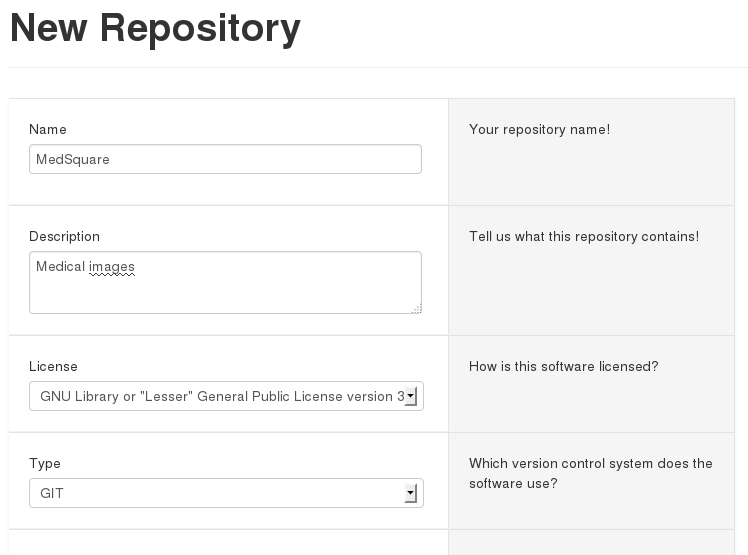
\includegraphics[width=\textwidth]{images/new-repository.png}
      \caption{Interface para criação de um novo repositório.}
      \label{fig:new-repository}
    \end{figure}

    Ao clicar em ``New repository'' entramos na criação do repositório a ser avaliado (figura \ref{fig:new-repository}). Alguns campos merecem destaque:
    \begin{itemize}
      \item\textbf{Type:} Tipo do repositório (também pode ser um zip ou tarball) onde o código está hospedado;
      \item\textbf{Address:} Endereço do repositório remoto ou o caminho absoluto no sistema de arquivos;
      \item\textbf{Process Period:} Periodicidade com a qual o código deve ser analizado pela ferramenta (diariamente, semanalmente etc);
      \item\textbf{Configuration:} Configuração de métricas que o usuário deseja utilizar para medir o código (pode ser escolhida dentre todas as configurações criadas pelos usuários).
    \end{itemize}
    Após preencher todos os campos e salvar o repositório, seu primeiro processamento será automaticamente ativado e o usuário será redirecionado para a página que exibe os resultados. Nela, ele poderá conferir dados do processamento (tempo gasto para o término de cada uma de suas fases) e navegar na árvore de módulos gerada, para que possa visualizar a nota, os resultados das métricas e suas interpretações para cada um deles (figura \ref{fig:results}). Além disso, ao clicar no nome de uma métrica calculada, um gráfico que representa a evolução dos seus valores ao longo do tempo será exibido.

    \begin{figure}[H]
      \centering
      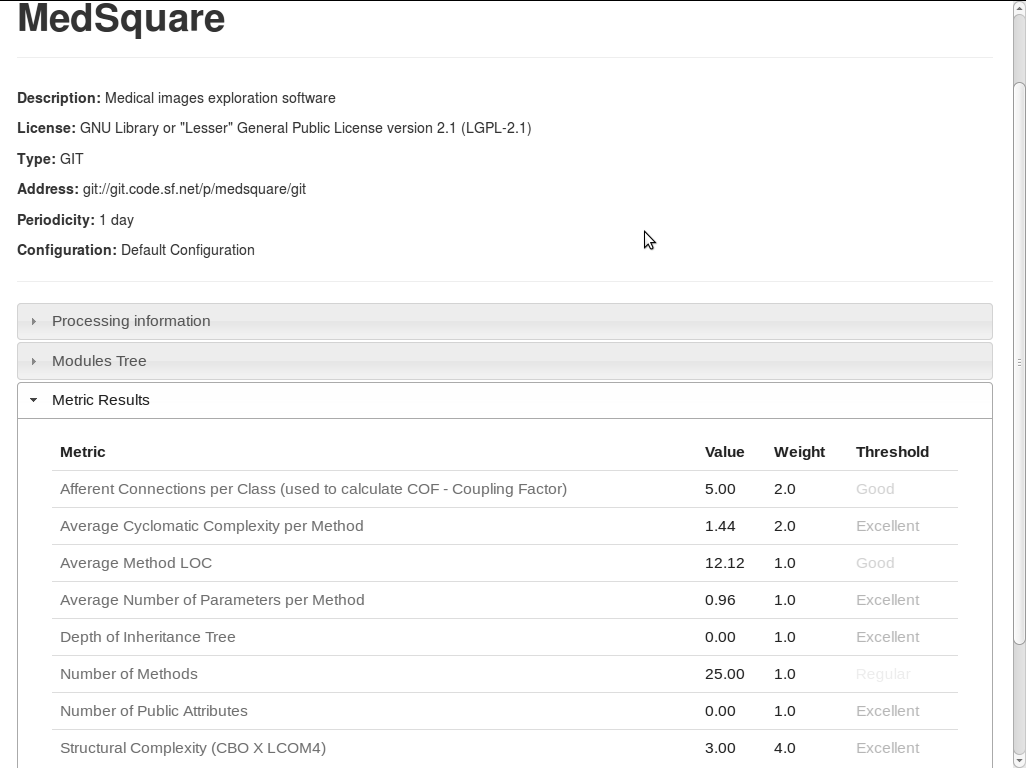
\includegraphics[width=\textwidth]{images/new-repository-results.png}
      \caption{Tela de visualização dos resultados do processamento do repositório.}
      \label{fig:results}
    \end{figure}

\section{Conclusão}
O Mezuro surge como uma potencial resposta para a falta de monitoramento e padronização de código-fonte e a necessidade de avaliação do mesmo, considerando que é um \textit{software} livre, altamente customizável, com suporte para muitas linguagens computacionais, interface amigável, que fornece histórico de processamentos e também com uma arquitetura planejada para incorporar novas funcionalidades.

\bibliographystyle{splncs03}
\bibliography{mezuro}
\end{document}
